% !TeX encoding=unicode
% !TeX spellcheck = de-DE

\chapter{Ergebnisse}
%
\begin{figure}
%% No H pT at Born, lpt_max = m_H / 2
\centering
%\begin{subfigure}[]{0.49\textwidth}
%	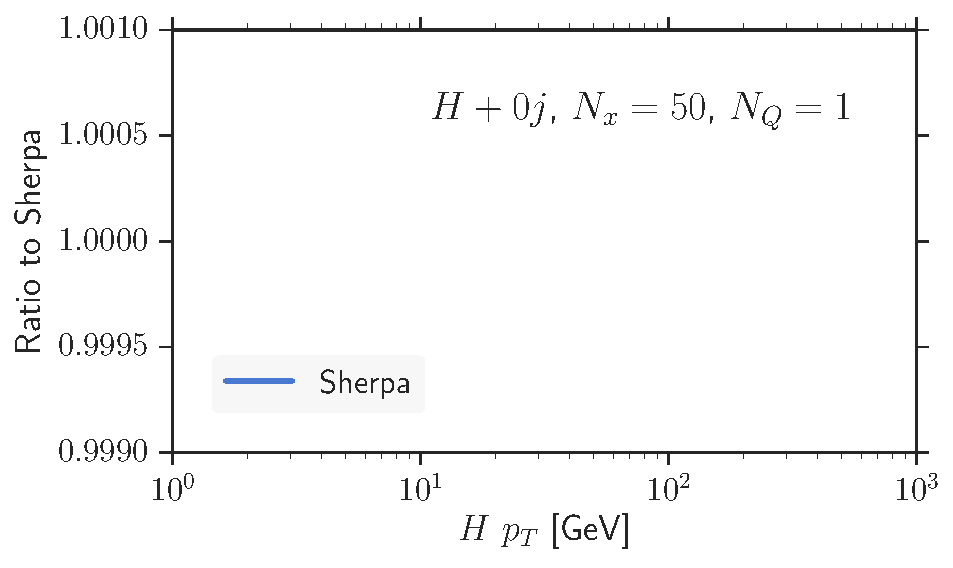
\includegraphics[width=\textwidth]{images/hb_hpt.pdf}
%\end{subfigure}
\hfill
\begin{subfigure}[]{0.49\textwidth}
	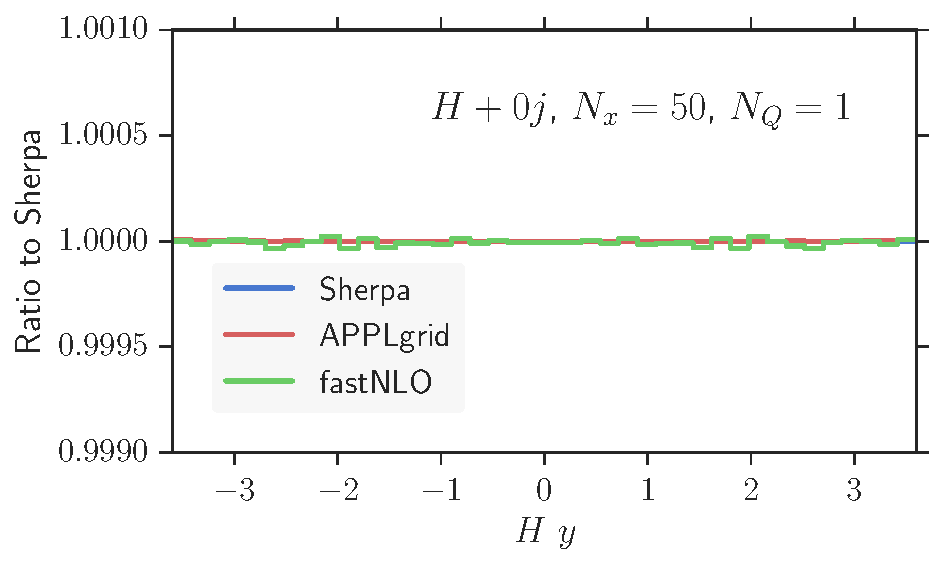
\includegraphics[width=\textwidth]{images/hb_hy.pdf}
\end{subfigure}

\begin{subfigure}[]{0.49\textwidth}
	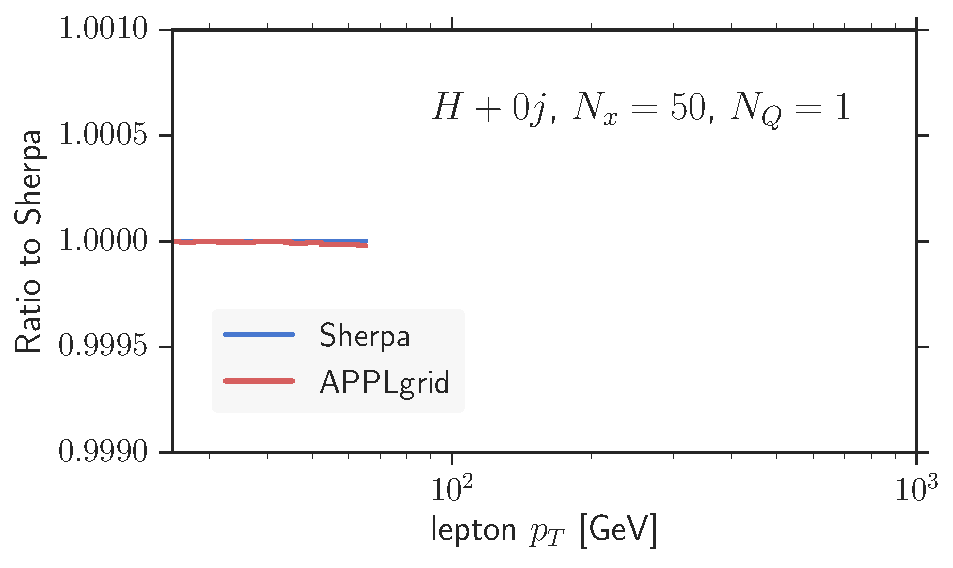
\includegraphics[width=\textwidth]{images/hb_lpt.pdf}
\end{subfigure}
\hfill
\begin{subfigure}[]{0.49\textwidth}
	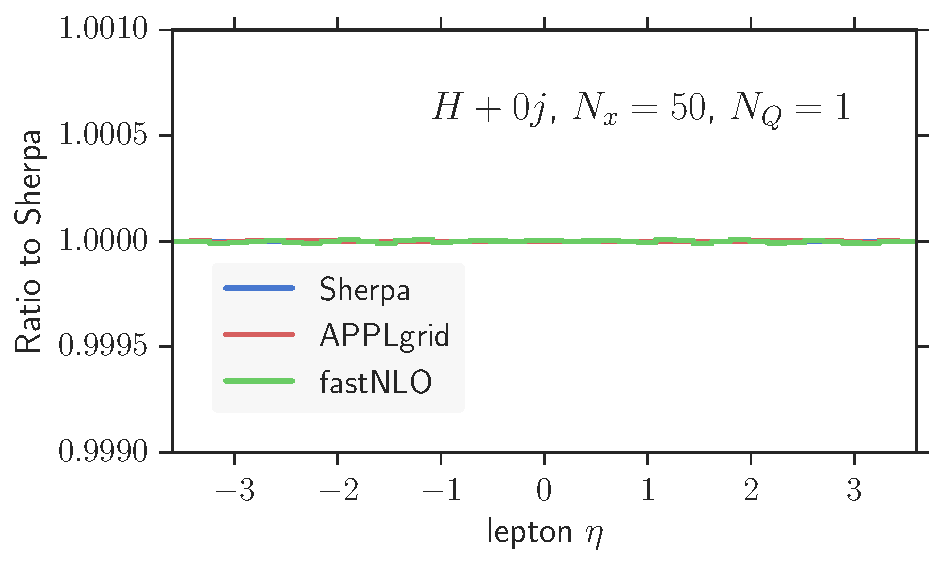
\includegraphics[width=\textwidth]{images/hb_leta.pdf}
\end{subfigure}
\caption{H B}
%\label{fig:bla}
\end{figure}
%
\begin{figure}
\centering
\begin{subfigure}[]{0.49\textwidth}
	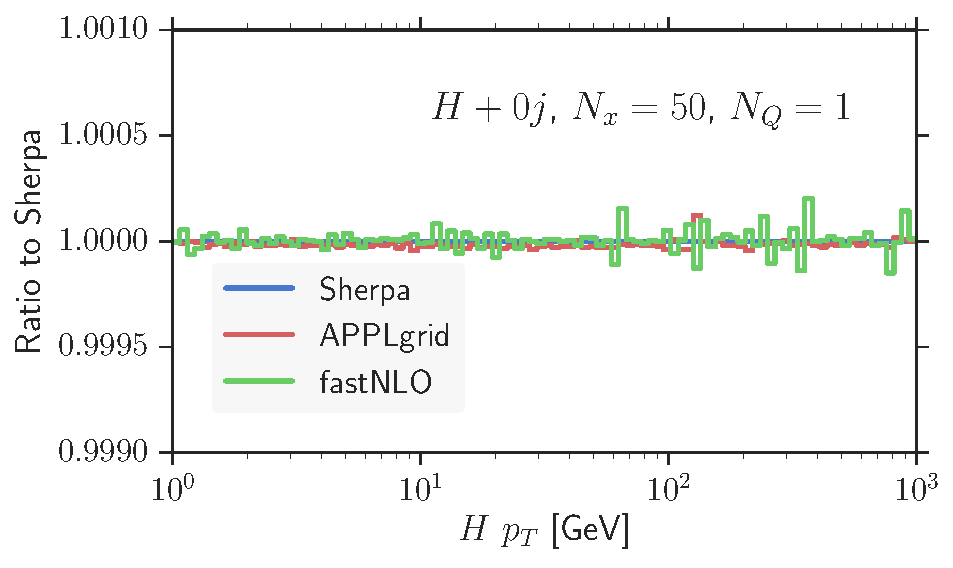
\includegraphics[width=\textwidth]{images/hrs_hpt.pdf}
\end{subfigure}
\hfill
\begin{subfigure}[]{0.49\textwidth}
	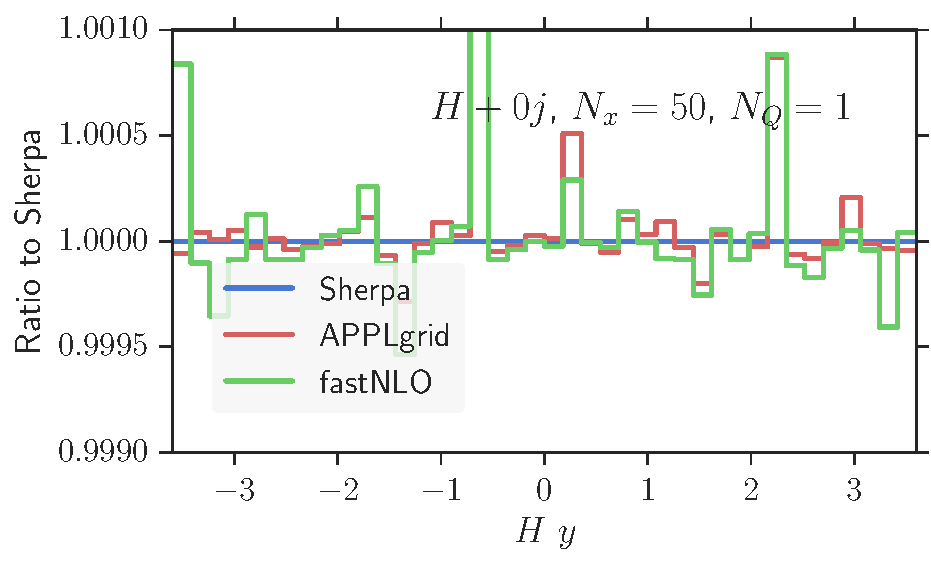
\includegraphics[width=\textwidth]{images/hrs_hy.pdf}
\end{subfigure}

\begin{subfigure}[]{0.49\textwidth}
	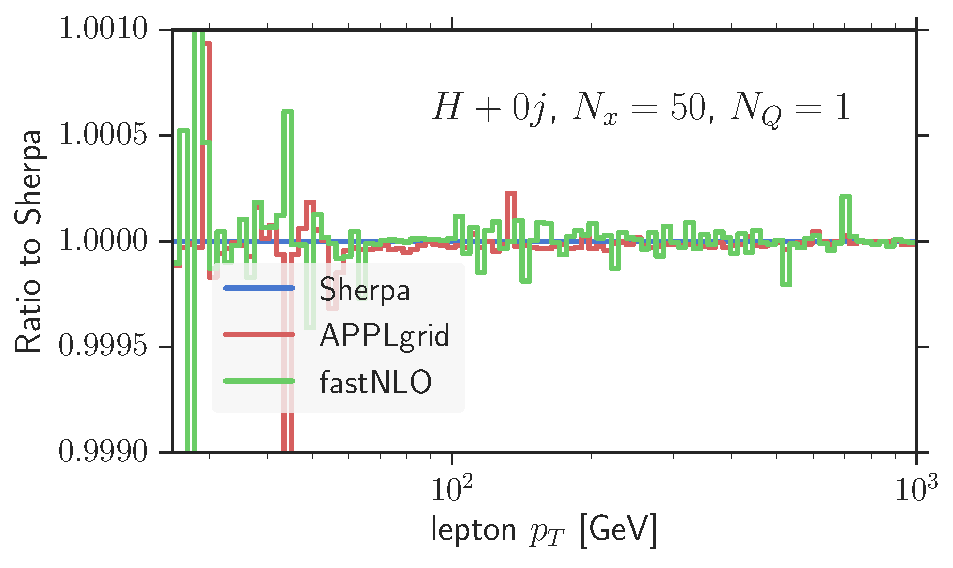
\includegraphics[width=\textwidth]{images/hrs_lpt.pdf}
\end{subfigure}
\hfill
\begin{subfigure}[]{0.49\textwidth}
	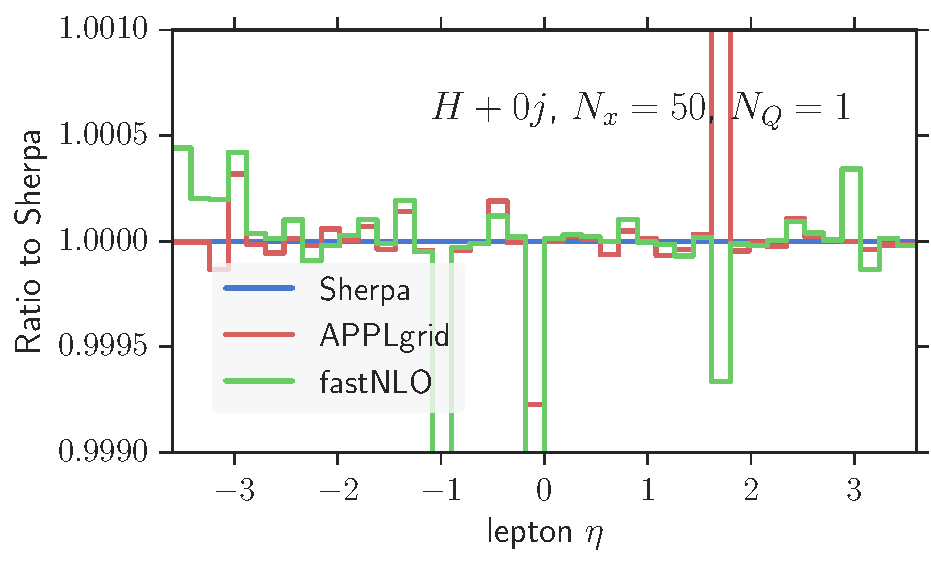
\includegraphics[width=\textwidth]{images/hrs_leta.pdf}
\end{subfigure}
\caption{H RS}
%\label{fig:bla}
\end{figure}
%
\begin{figure}
\centering
%\begin{subfigure}[]{0.49\textwidth}
%	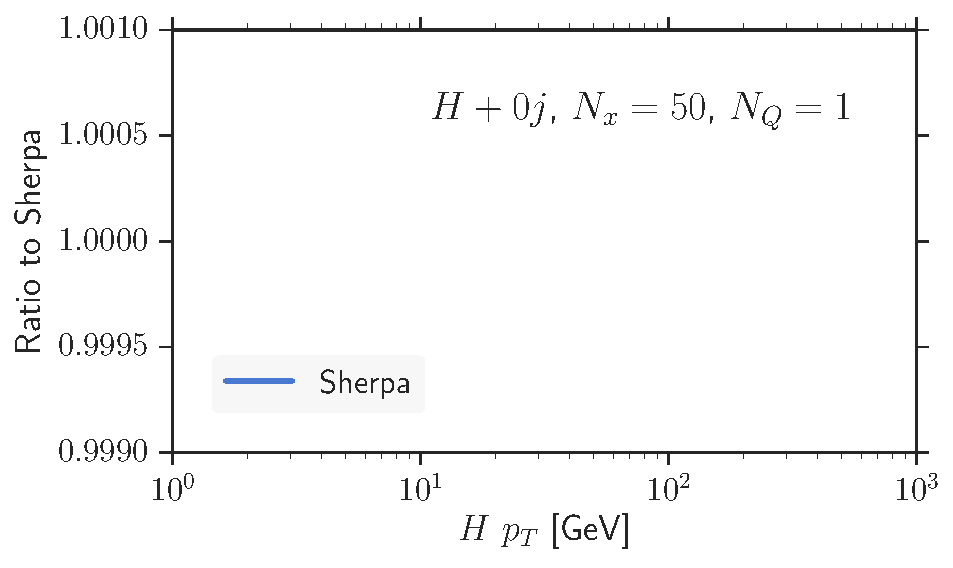
\includegraphics[width=\textwidth]{images/hvi_hpt.pdf}
%\end{subfigure}
\hfill
\begin{subfigure}[]{0.49\textwidth}
	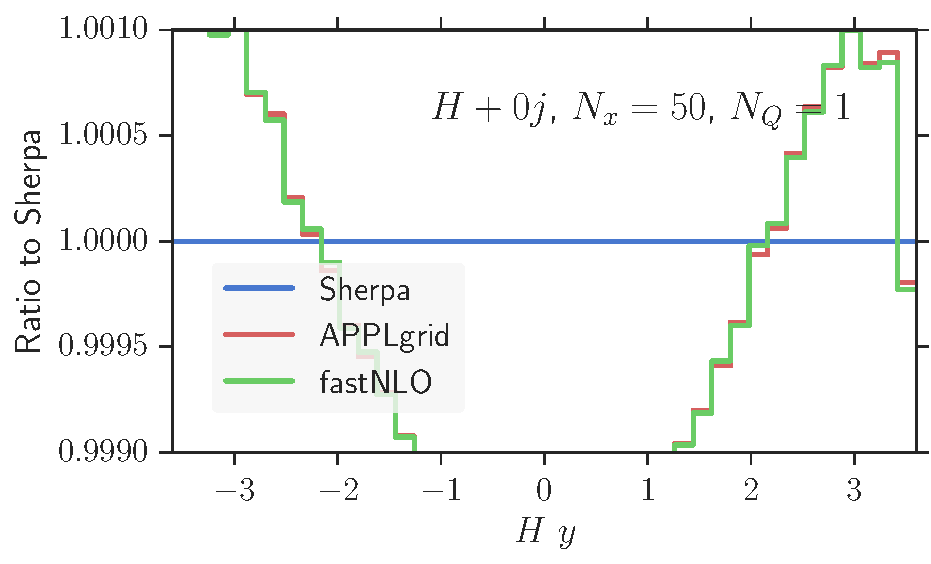
\includegraphics[width=\textwidth]{images/hvi_hy.pdf}
\end{subfigure}

\begin{subfigure}[]{0.49\textwidth}
	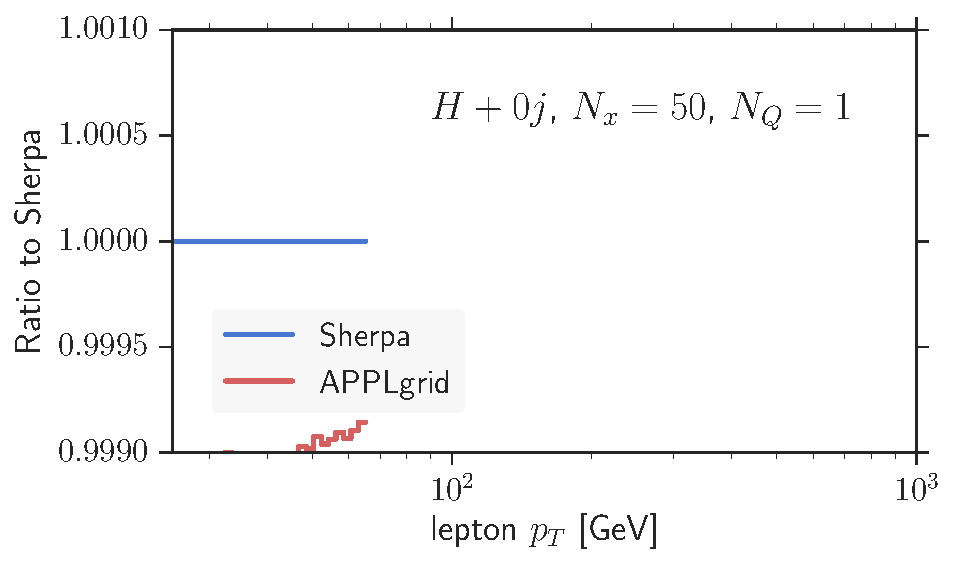
\includegraphics[width=\textwidth]{images/hvi_lpt.pdf}
\end{subfigure}
\hfill
\begin{subfigure}[]{0.49\textwidth}
	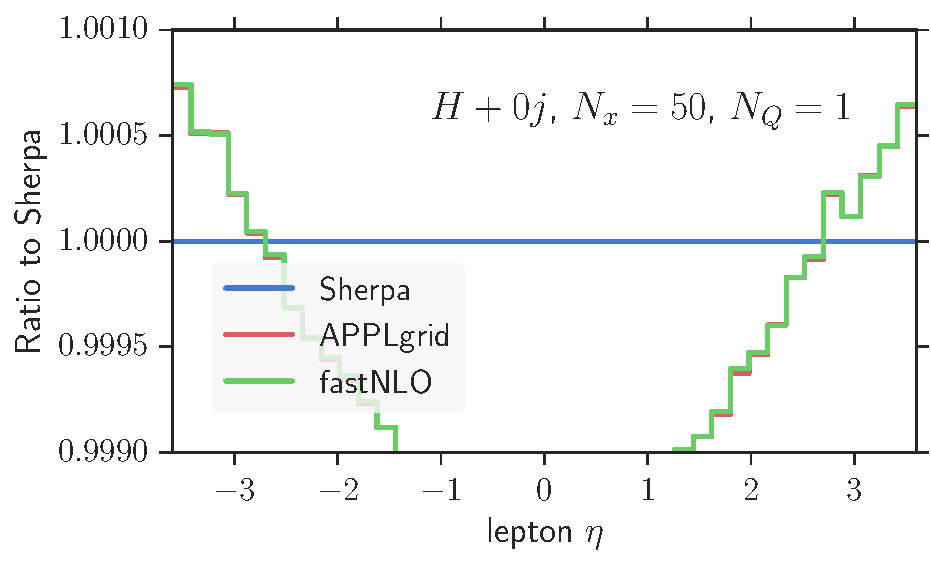
\includegraphics[width=\textwidth]{images/hvi_leta.pdf}
\end{subfigure}
\caption{H VI}
%\label{fig:bla}
\end{figure}
%
\begin{figure}
\centering
\begin{subfigure}[]{0.49\textwidth}
	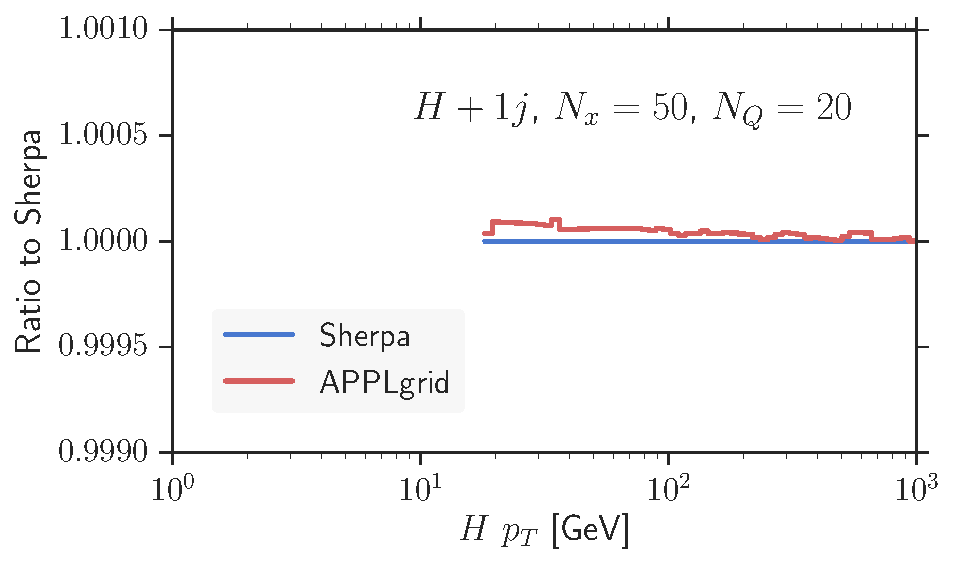
\includegraphics[width=\textwidth]{images/hjb_hpt.pdf}
\end{subfigure}
\hfill
\begin{subfigure}[]{0.49\textwidth}
	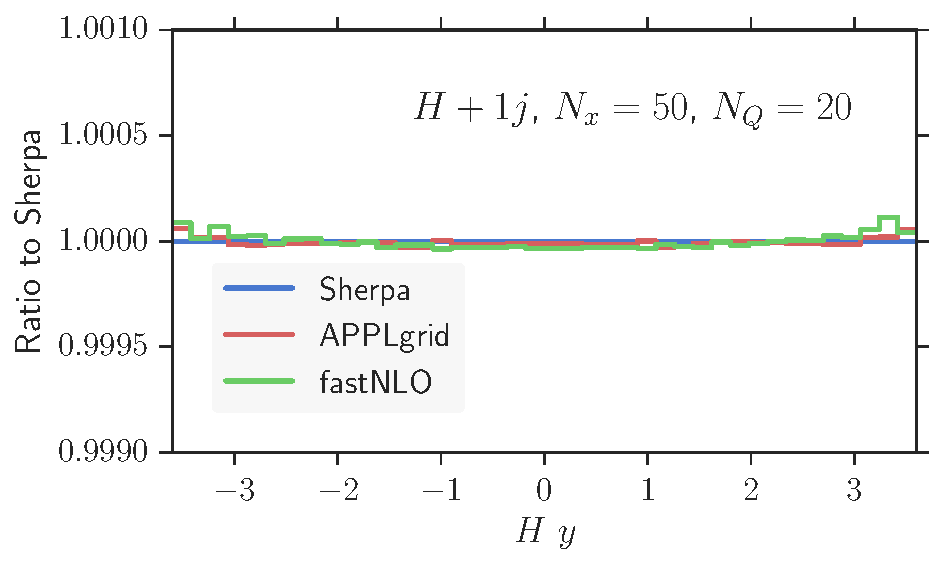
\includegraphics[width=\textwidth]{images/hjb_hy.pdf}
\end{subfigure}

\begin{subfigure}[]{0.49\textwidth}
	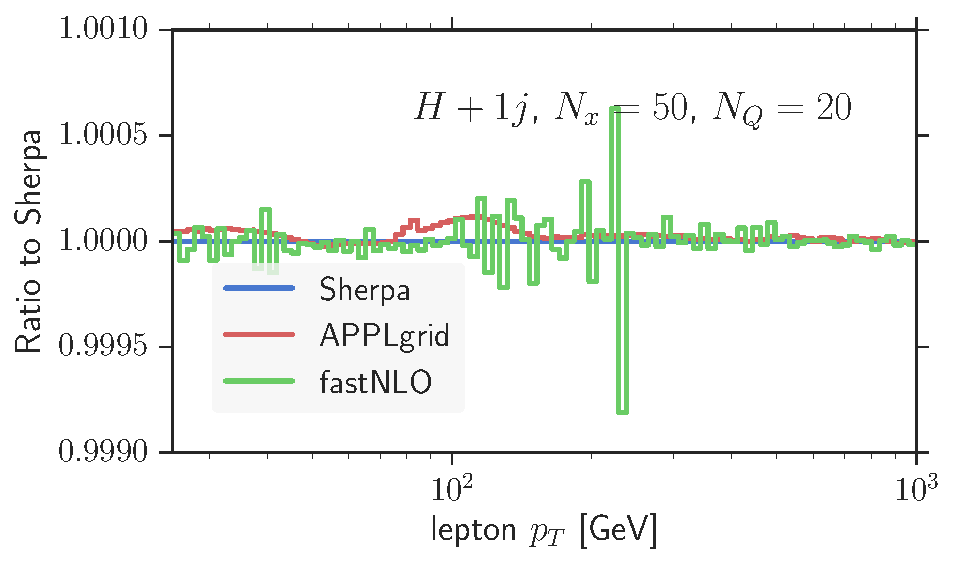
\includegraphics[width=\textwidth]{images/hjb_lpt.pdf}
\end{subfigure}
\hfill
\begin{subfigure}[]{0.49\textwidth}
	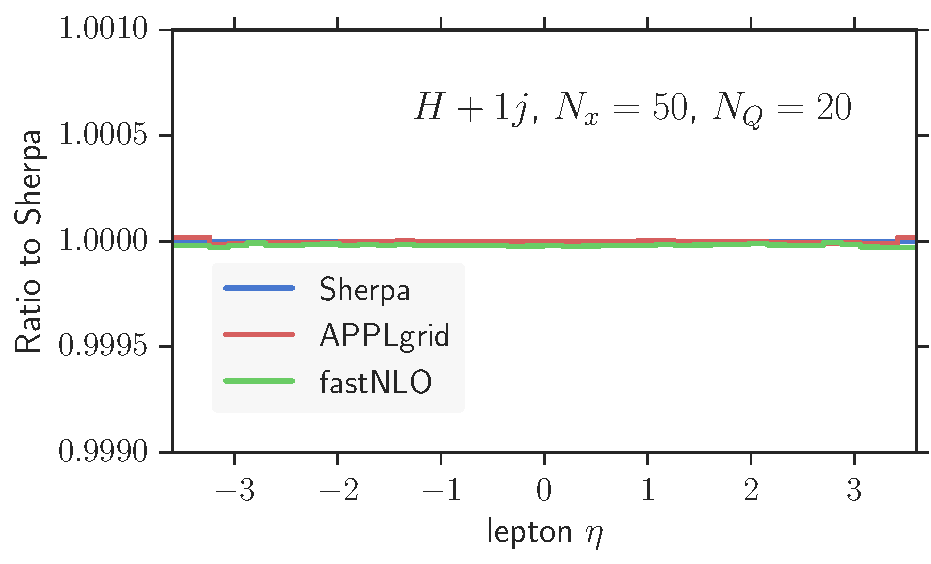
\includegraphics[width=\textwidth]{images/hjb_leta.pdf}
\end{subfigure}
\caption{Hj B}
%\label{fig:bla}
\end{figure}
%
\begin{figure}
\centering
\begin{subfigure}[]{0.49\textwidth}
	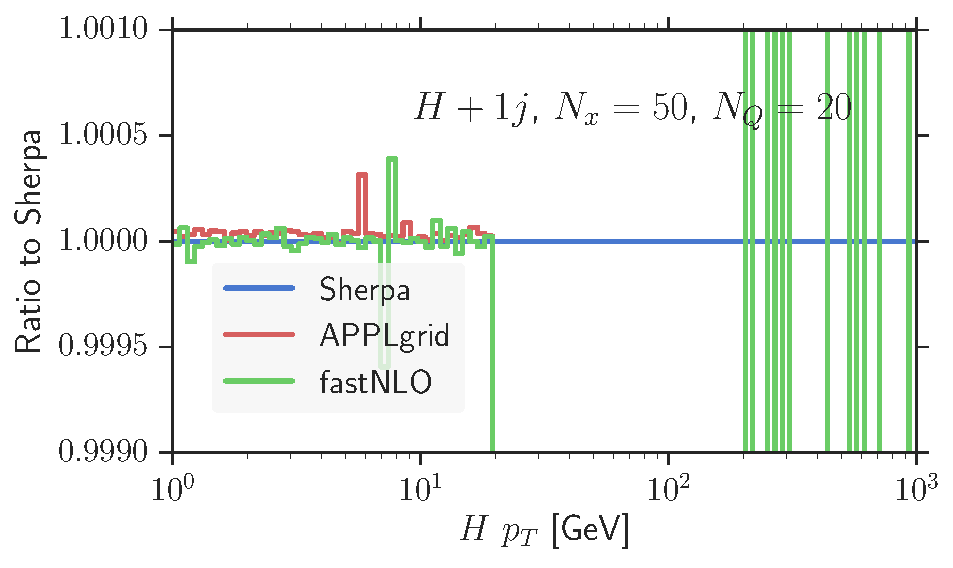
\includegraphics[width=\textwidth]{images/hjrs_hpt.pdf}
\end{subfigure}
\hfill
\begin{subfigure}[]{0.49\textwidth}
	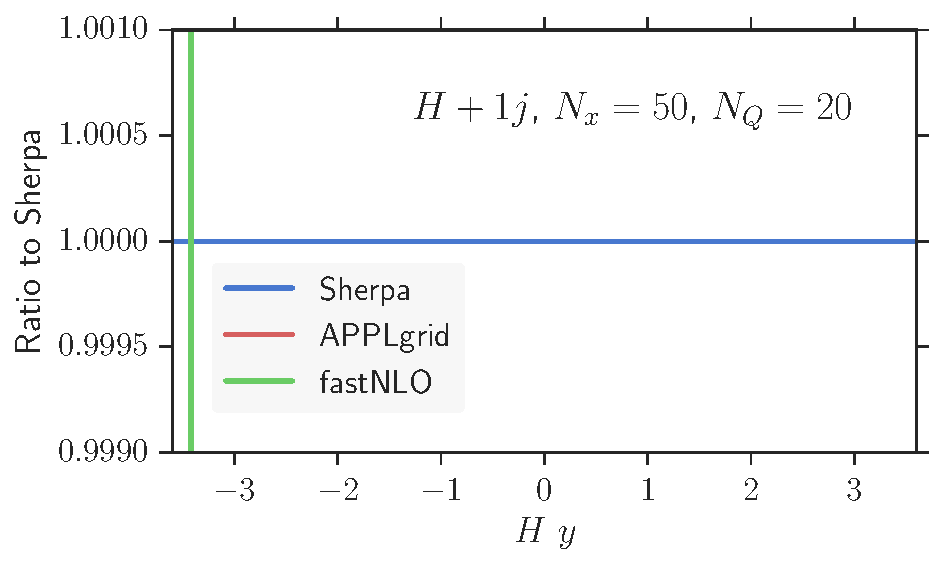
\includegraphics[width=\textwidth]{images/hjrs_hy.pdf}
\end{subfigure}

\begin{subfigure}[]{0.49\textwidth}
	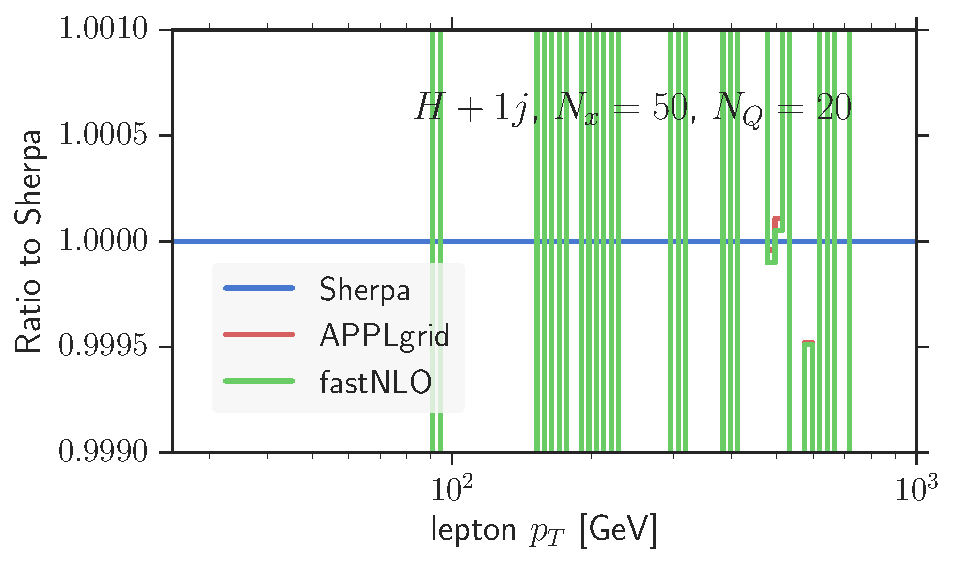
\includegraphics[width=\textwidth]{images/hjrs_lpt.pdf}
\end{subfigure}
\hfill
\begin{subfigure}[]{0.49\textwidth}
	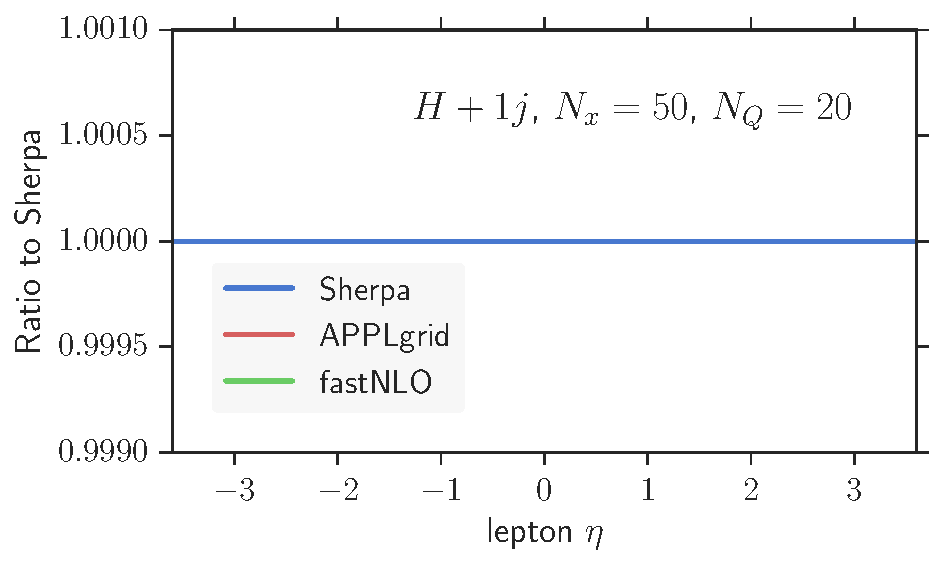
\includegraphics[width=\textwidth]{images/hjrs_leta.pdf}
\end{subfigure}
\caption{Hj RS}
%\label{fig:bla}
\end{figure}
%
\begin{figure}
\centering
\begin{subfigure}[]{0.49\textwidth}
	%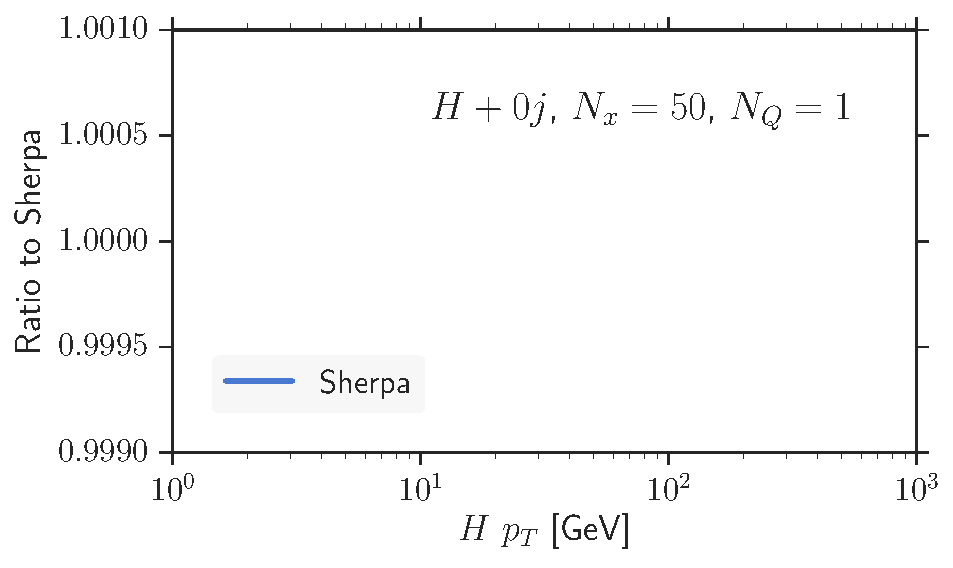
\includegraphics[width=\textwidth]{images/hb_hpt.pdf}
	
\includegraphics[width=\textwidth]{images/dummy.pdf}
\end{subfigure}
\hfill
\begin{subfigure}[]{0.49\textwidth}
	%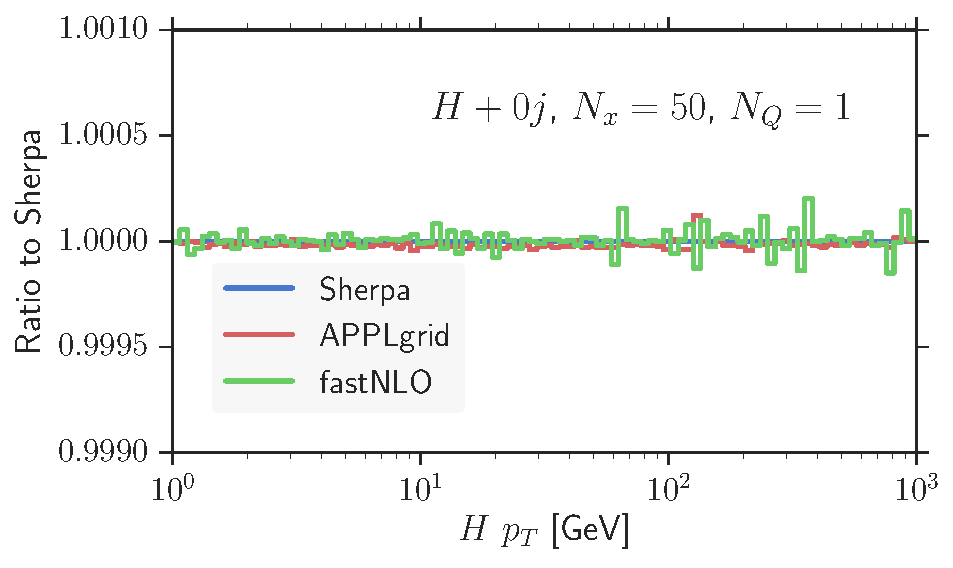
\includegraphics[width=\textwidth]{images/hrs_hpt.pdf}
	
\includegraphics[width=\textwidth]{images/dummy.pdf}
\end{subfigure}

\begin{subfigure}[]{0.49\textwidth}
	%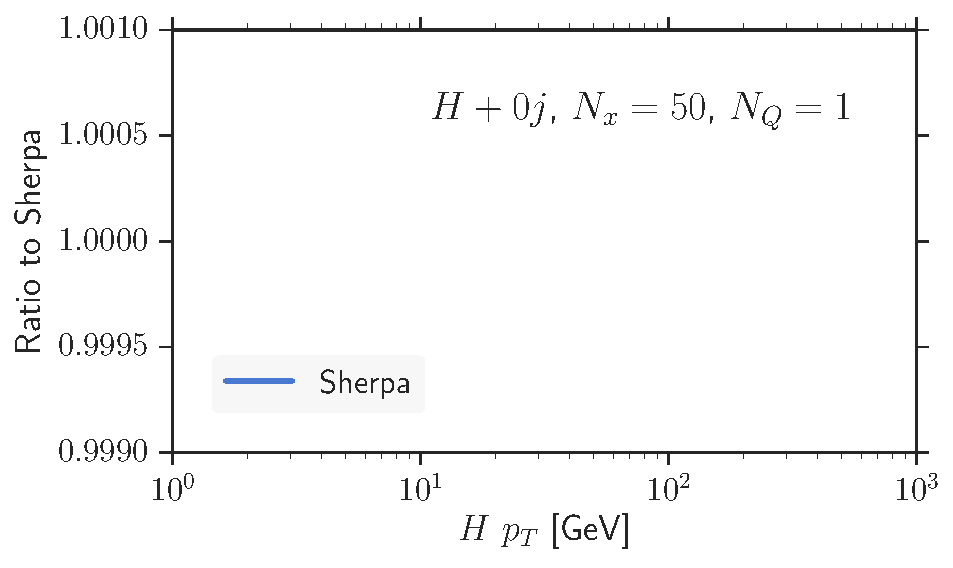
\includegraphics[width=\textwidth]{images/hvi_hpt.pdf}
	
\includegraphics[width=\textwidth]{images/dummy.pdf}
\end{subfigure}
\hfill
\begin{subfigure}[]{0.49\textwidth}
	%\includegraphics[width=\textwidth]{images/hb_hptpeak.pdf}
	
\includegraphics[width=\textwidth]{images/dummy.pdf}
\end{subfigure}
\caption{Hj VI}
%\label{fig:bla}
\end{figure}
%
\begin{figure}
\centering
\begin{subfigure}[]{0.49\textwidth}
	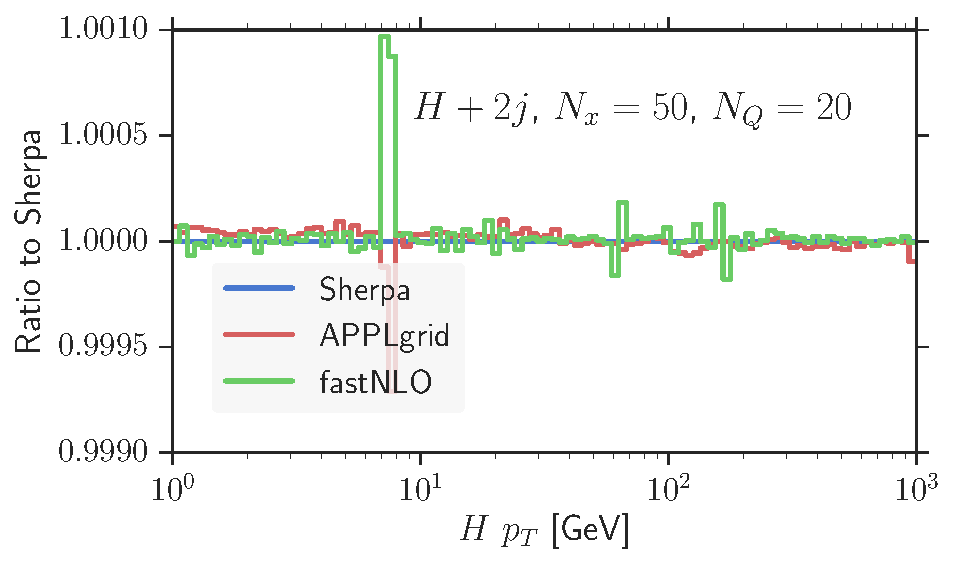
\includegraphics[width=\textwidth]{images/hjjb_hpt.pdf}
\end{subfigure}
\hfill
\begin{subfigure}[]{0.49\textwidth}
	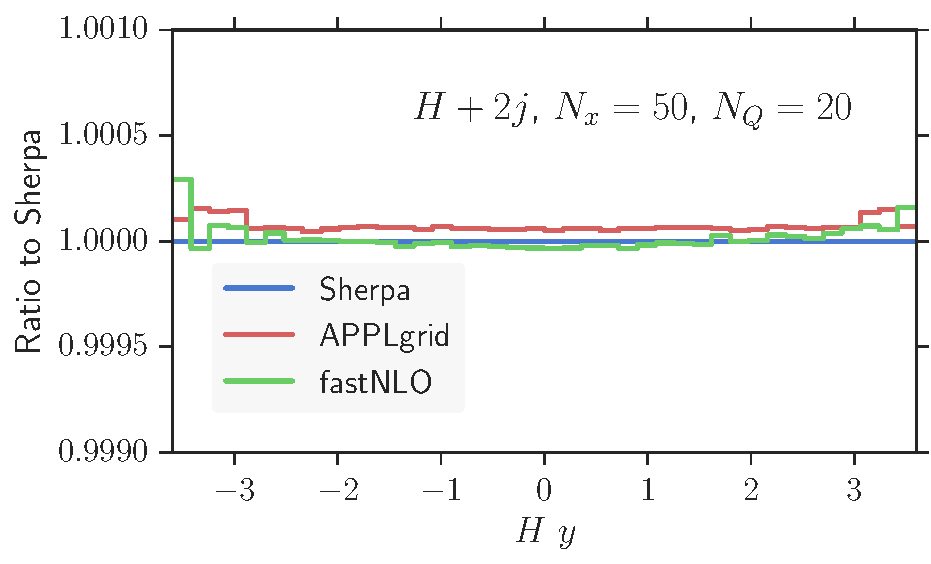
\includegraphics[width=\textwidth]{images/hjjb_hy.pdf}
\end{subfigure}

\begin{subfigure}[]{0.49\textwidth}
	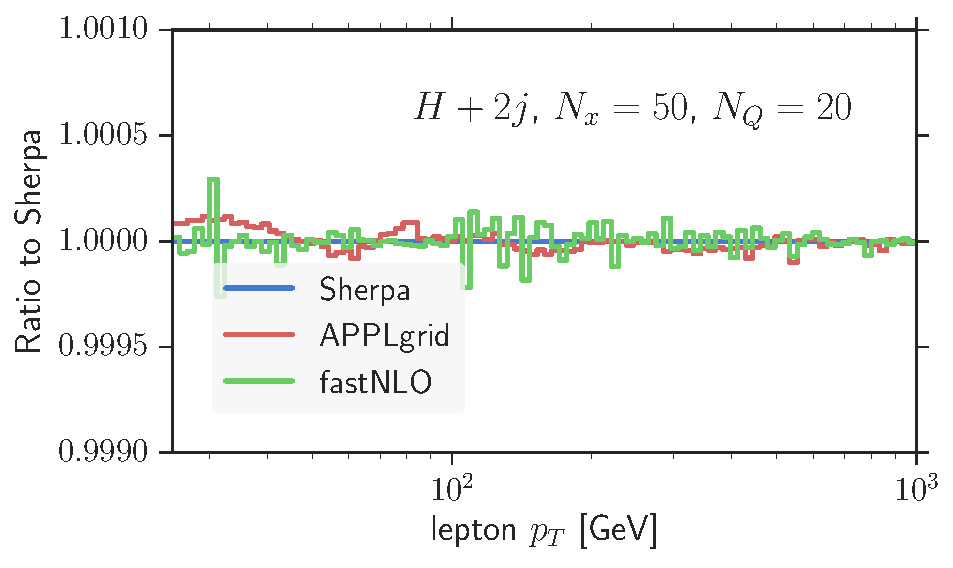
\includegraphics[width=\textwidth]{images/hjjb_lpt.pdf}
\end{subfigure}
\hfill
\begin{subfigure}[]{0.49\textwidth}
	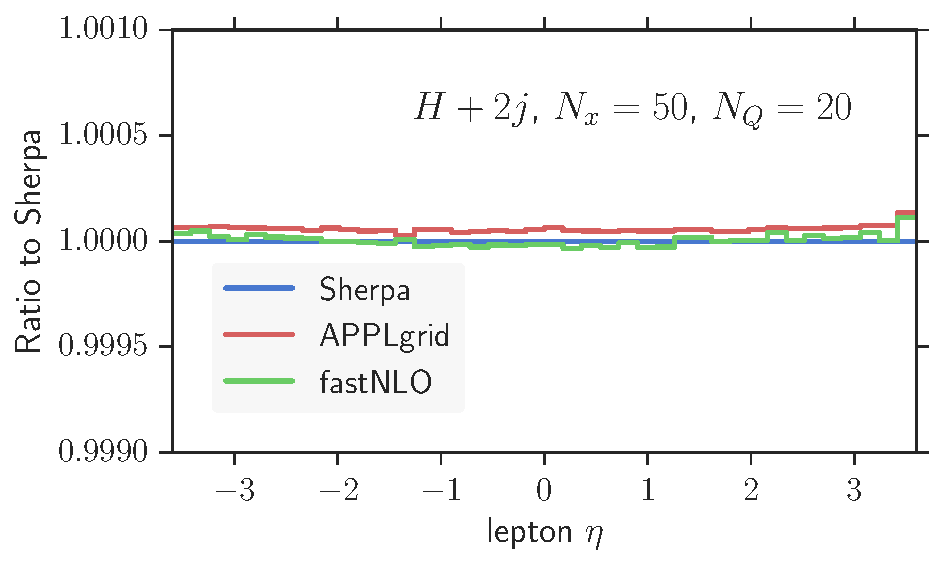
\includegraphics[width=\textwidth]{images/hjjb_leta.pdf}
\end{subfigure}
\caption{Hjj B}
%\label{fig:bla}
\end{figure}
%
\begin{figure}
\centering
\begin{subfigure}[]{0.49\textwidth}
	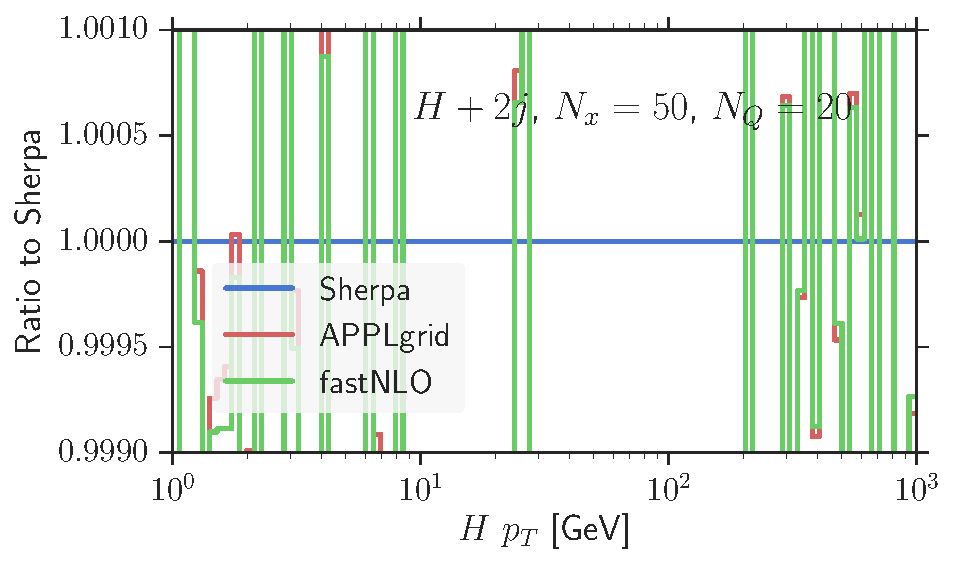
\includegraphics[width=\textwidth]{images/hjjrs_hpt.pdf}
\end{subfigure}
\hfill
\begin{subfigure}[]{0.49\textwidth}
	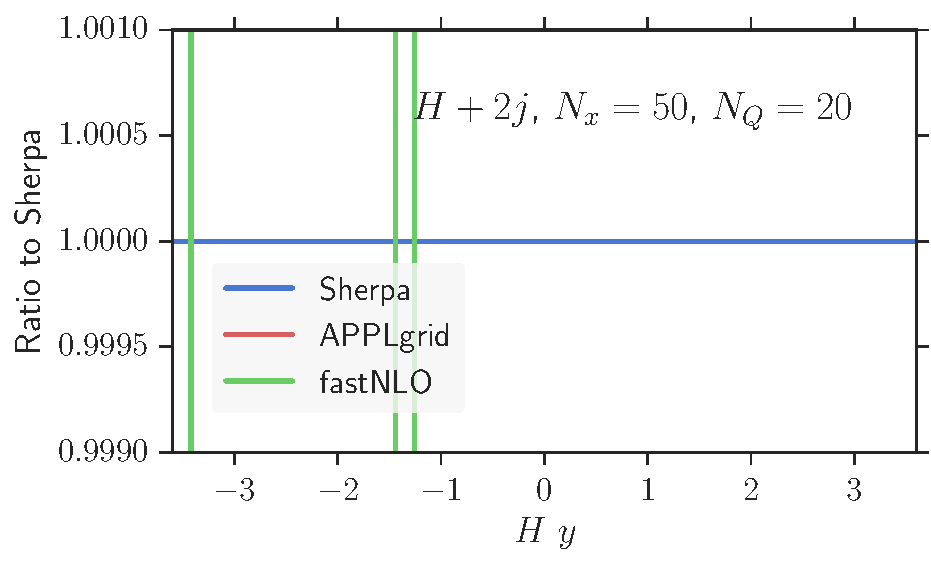
\includegraphics[width=\textwidth]{images/hjjrs_hy.pdf}
\end{subfigure}

\begin{subfigure}[]{0.49\textwidth}
	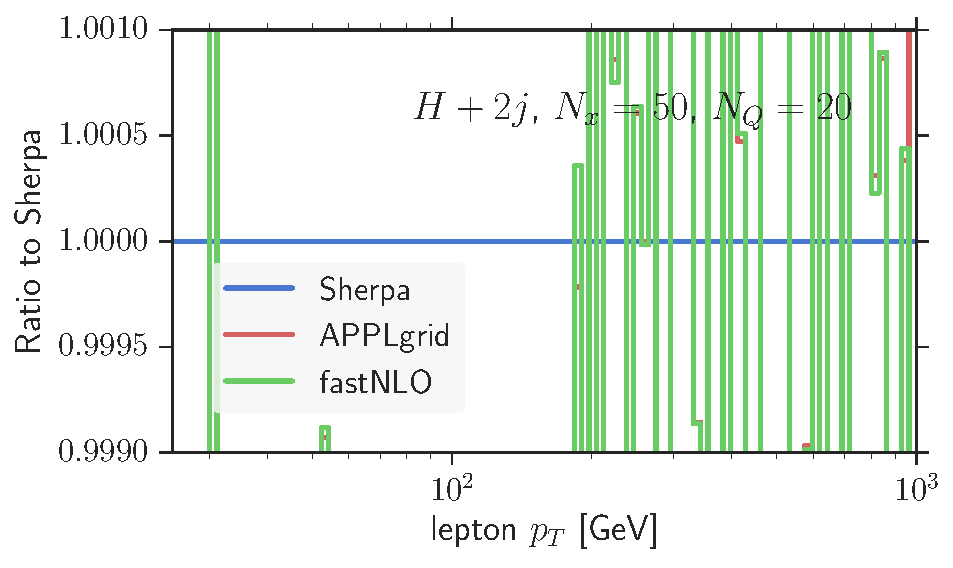
\includegraphics[width=\textwidth]{images/hjjrs_lpt.pdf}
\end{subfigure}
\hfill
\begin{subfigure}[]{0.49\textwidth}
	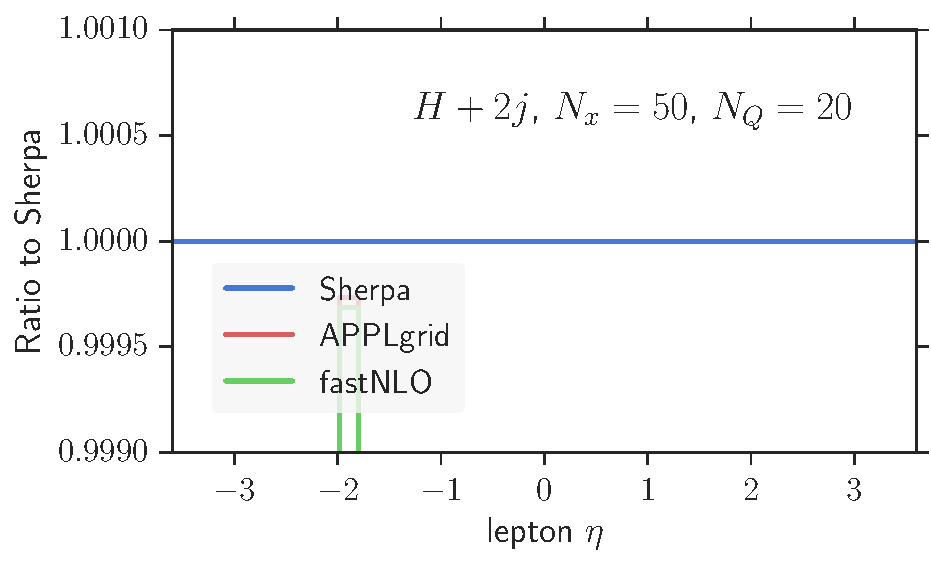
\includegraphics[width=\textwidth]{images/hjjrs_leta.pdf}
\end{subfigure}
\caption{Hjj RS}
%\label{fig:bla}
\end{figure}
%
\begin{figure}
\centering
\begin{subfigure}[]{0.49\textwidth}
	%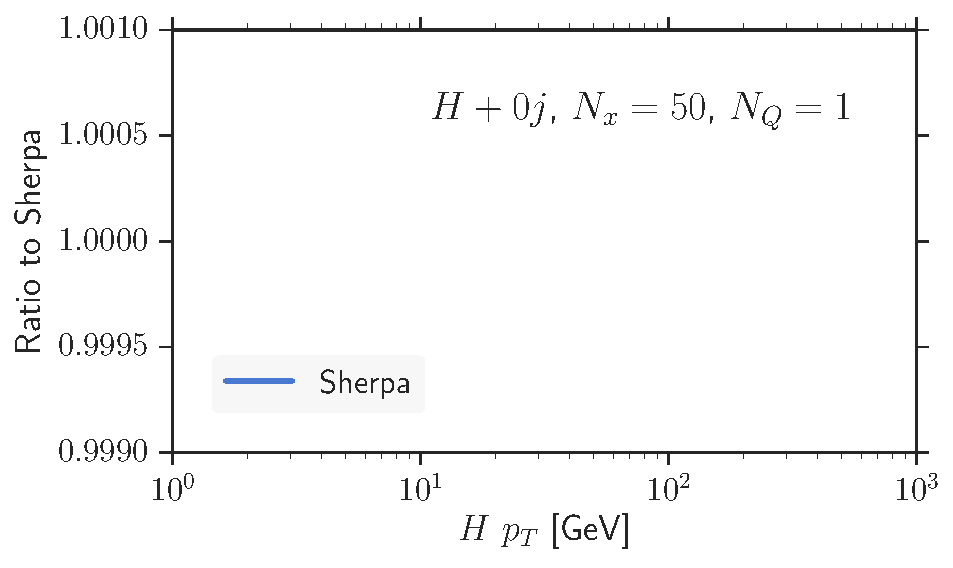
\includegraphics[width=\textwidth]{images/hb_hpt.pdf}
	
\includegraphics[width=\textwidth]{images/dummy.pdf}
\end{subfigure}
\hfill
\begin{subfigure}[]{0.49\textwidth}
	%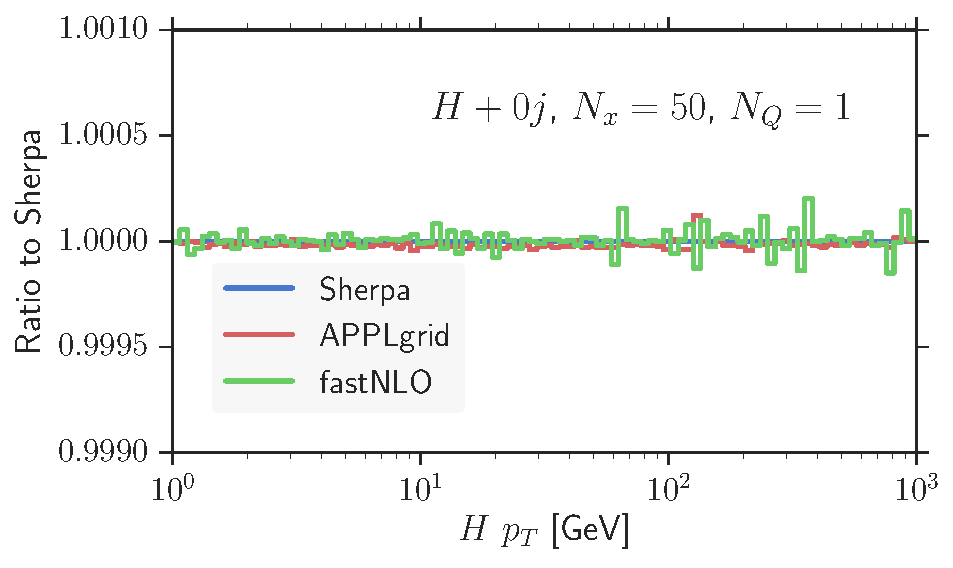
\includegraphics[width=\textwidth]{images/hrs_hpt.pdf}
	
\includegraphics[width=\textwidth]{images/dummy.pdf}
\end{subfigure}

\begin{subfigure}[]{0.49\textwidth}
	%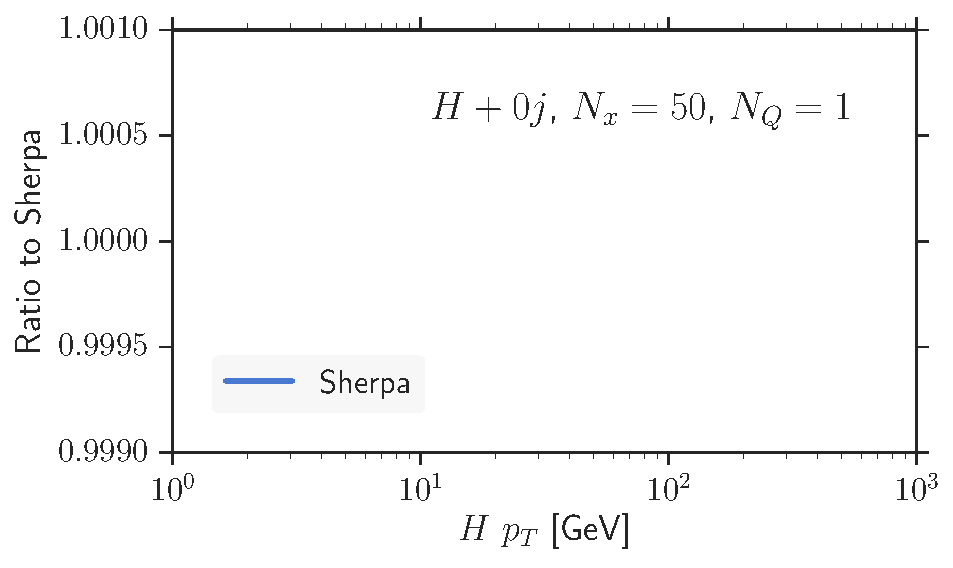
\includegraphics[width=\textwidth]{images/hvi_hpt.pdf}
	
\includegraphics[width=\textwidth]{images/dummy.pdf}
\end{subfigure}
\hfill
\begin{subfigure}[]{0.49\textwidth}
	%\includegraphics[width=\textwidth]{images/hb_hptpeak.pdf}
	
\includegraphics[width=\textwidth]{images/dummy.pdf}
\end{subfigure}
\caption{Hjj VI}
%\label{fig:bla}
\end{figure}
%


%
\begin{figure}
\centering
\begin{subfigure}[]{0.49\textwidth}
	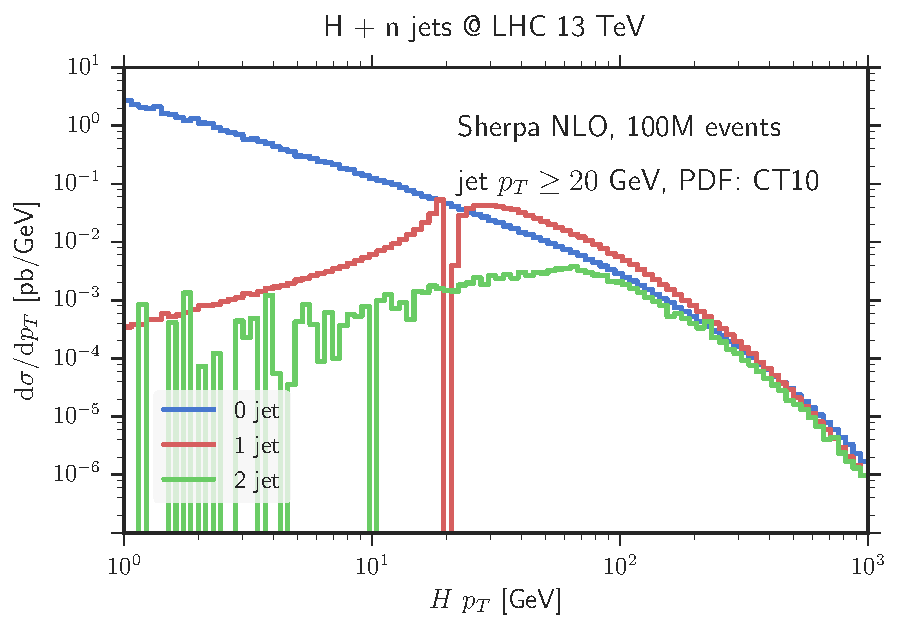
\includegraphics[width=\textwidth]{images/cmp100m_nlo_hpt.pdf}
\end{subfigure}
\hfill
\begin{subfigure}[]{0.49\textwidth}
	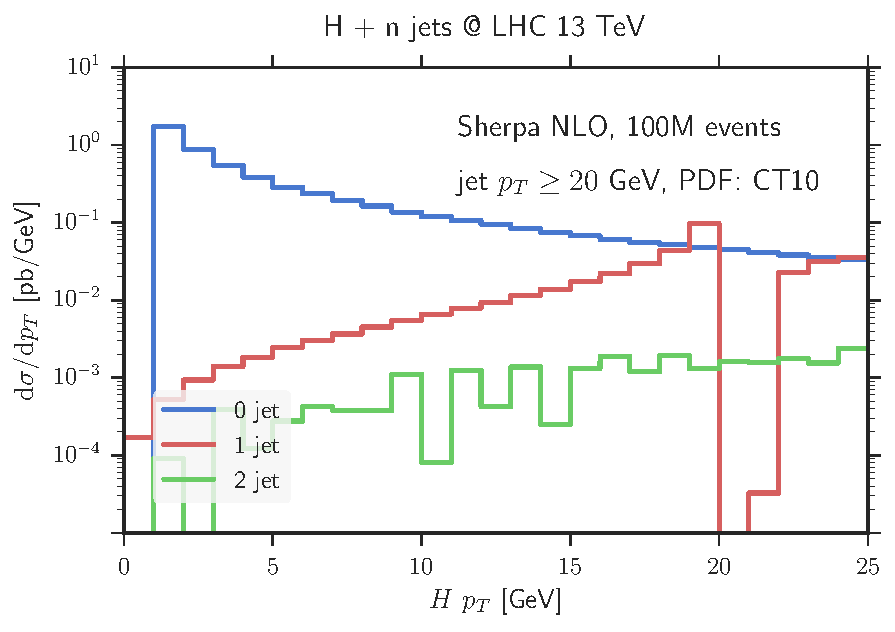
\includegraphics[width=\textwidth]{images/cmp100m_nlo_hptpeak.pdf}
\end{subfigure}
\caption{H pT NLO (0,1,2) jets}
%\label{fig:bla}
\end{figure}
%
\begin{figure}
\centering
\begin{subfigure}[]{0.49\textwidth}
	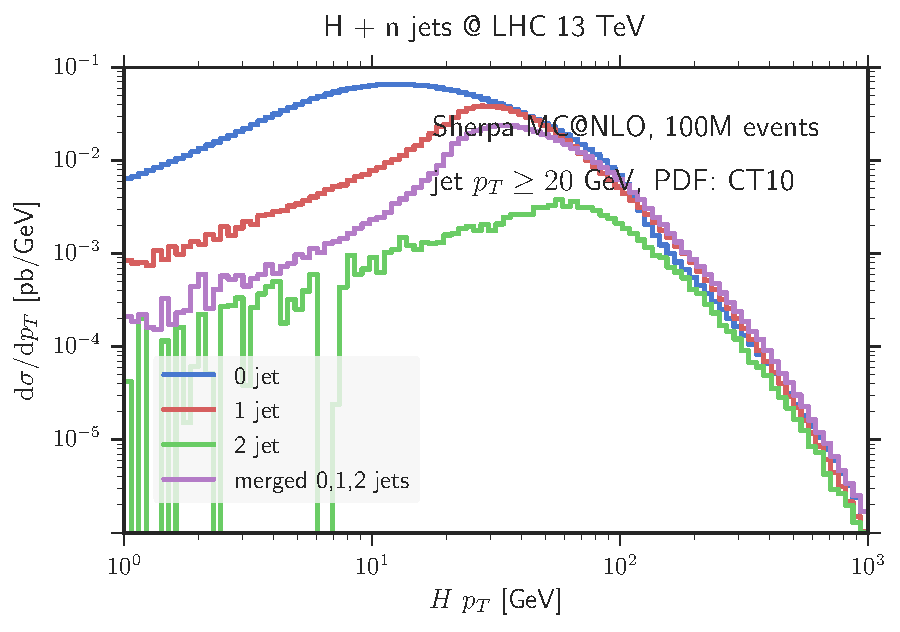
\includegraphics[width=\textwidth]{images/cmp100m_mcatnlo_hpt.pdf}
\end{subfigure}
\hfill
\begin{subfigure}[]{0.49\textwidth}
	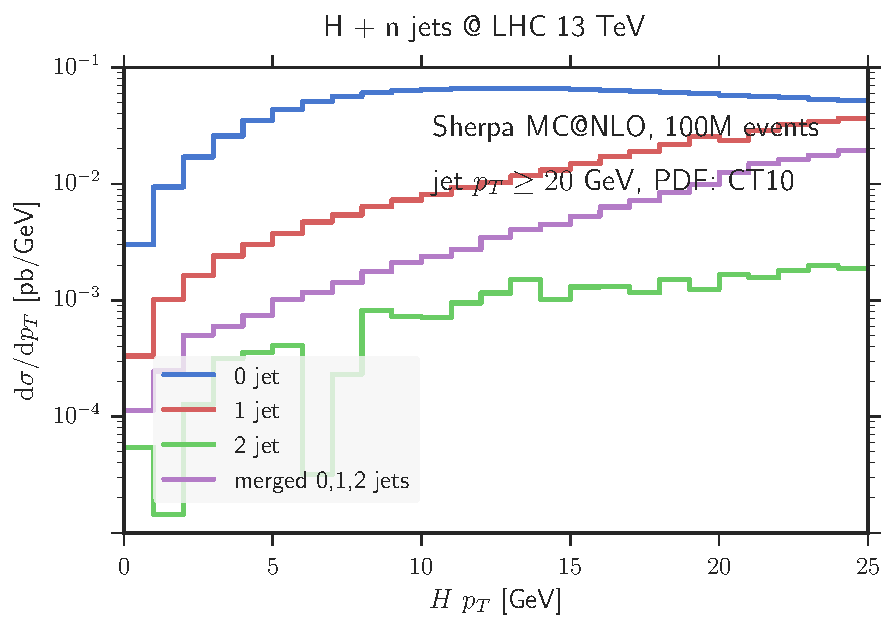
\includegraphics[width=\textwidth]{images/cmp100m_mcatnlo_hptpeak.pdf}
\end{subfigure}
\caption{H pT MCatNLO (0,1,2) jets}
%\label{fig:bla}
\end{figure}
%


%
\begin{figure}
\centering
\begin{subfigure}[]{0.49\textwidth}
	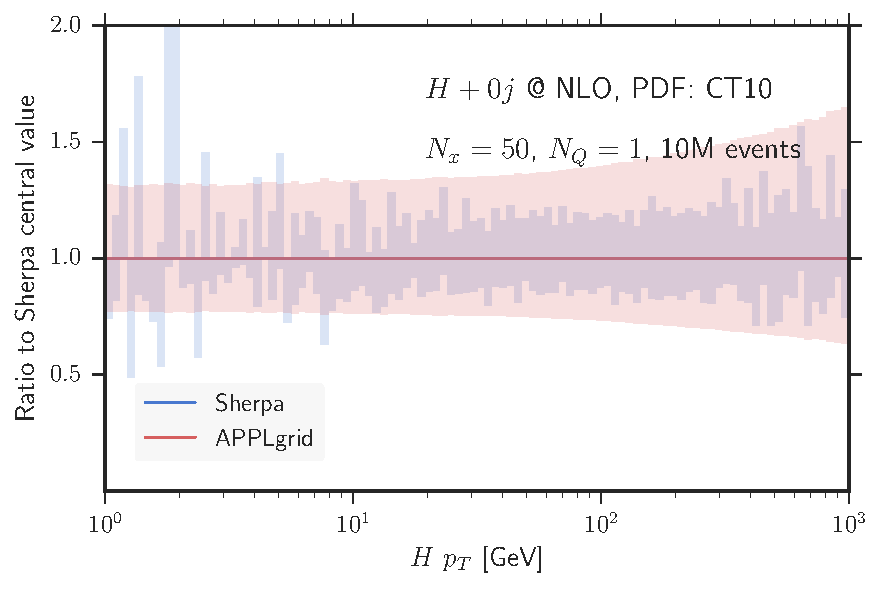
\includegraphics[width=\textwidth]{images/plot_scalesvar_band_hpt.pdf}
	\caption{10M events}
\end{subfigure}
\hfill
\begin{subfigure}[]{0.49\textwidth}
	
\includegraphics[width=\textwidth]{images/dummy.pdf}
	\caption{100M events}
\end{subfigure}
\caption{Scale variations band}
%\label{fig:bla}
\end{figure}
%
\begin{figure}
\centering
\begin{subfigure}[]{0.49\textwidth}
	\includegraphics[width=\textwidth]{images/plot_scalesvar_ratio_hpt.pdf}
	\caption{10M events}
\end{subfigure}
\hfill
\begin{subfigure}[]{0.49\textwidth}
	\includegraphics[width=\textwidth]{images/dummy.pdf}
	\caption{100M events}
\end{subfigure}
\caption{Scale variations ratio}
%\label{fig:bla}
\end{figure}
%
